\documentclass[pdflatex,sn-aps,referee,lineno]{sn-jnl}% APS reference style; double spacing, line numbers

\usepackage{graphicx}%
\usepackage{multirow}%
\usepackage{amsmath,amssymb,amsfonts}%
\usepackage{xcolor}%
\usepackage{booktabs}%
\usepackage{array}%
\usepackage{adjustbox}%
\usepackage{tikz}%
\usetikzlibrary{arrows.meta,positioning,fit,backgrounds}%

\graphicspath{{figures/}}

% generated by make_tables_cls.py - do not edit
\newcommand{\ClsAOurs}{0.589}
\newcommand{\ClsALab}{0.572}
\newcommand{\ClsAOwn}{0.607}
\newcommand{\ClsAInput}{0.552}
\newcommand{\ClsASingle}{0.275}
\newcommand{\ClsAOursRaw}{0.414}
\newcommand{\ClsALabRaw}{0.374}
\newcommand{\ClsAScanned}{0.562}
\newcommand{\ClsALabScanned}{0.547}
\newcommand{\ClsACars}{8}
\newcommand{\ClsADLab}{$+0.017$ $[-0.071, +0.093]$}
\newcommand{\ClsADInput}{$+0.037$ $[-0.069, +0.130]$}
\newcommand{\ClsADOwn}{$-0.018$ $[-0.068, +0.021]$}
\newcommand{\ClsADSingle}{$+0.314$ $[+0.229, +0.400]$}
\newcommand{\ClsAWinsLab}{6}
\newcommand{\ClsALerr}{0.52}
\newcommand{\ClsAWerr}{0.08}
\newcommand{\ClsAHerr}{0.22}
\newcommand{\ClsAFieldErr}{23}
\newcommand{\ClsAHeading}{3.2}
\newcommand{\ClsAAlong}{0.82}
\newcommand{\ClsAAcross}{0.23}
\newcommand{\ClsASide}{8}
\newcommand{\ClsAFilled}{0.39}
\newcommand{\ClsBOurs}{0.507}
\newcommand{\ClsBLab}{0.508}
\newcommand{\ClsBOwn}{0.484}
\newcommand{\ClsBInput}{0.504}
\newcommand{\ClsBSingle}{0.401}
\newcommand{\ClsBOursRaw}{0.357}
\newcommand{\ClsBLabRaw}{0.322}
\newcommand{\ClsBScanned}{0.481}
\newcommand{\ClsBLabScanned}{0.488}
\newcommand{\ClsBCars}{9}
\newcommand{\ClsBDLab}{$-0.001$ $[-0.080, +0.058]$}
\newcommand{\ClsBDInput}{$+0.002$ $[-0.063, +0.055]$}
\newcommand{\ClsBDOwn}{$+0.022$ $[-0.019, +0.057]$}
\newcommand{\ClsBDSingle}{$+0.106$ $[+0.022, +0.184]$}
\newcommand{\ClsBWinsLab}{7}
\newcommand{\ClsBLerr}{0.43}
\newcommand{\ClsBWerr}{0.19}
\newcommand{\ClsBHerr}{0.23}
\newcommand{\ClsBFieldErr}{34}
\newcommand{\ClsBHeading}{1.3}
\newcommand{\ClsBAlong}{2.22}
\newcommand{\ClsBAcross}{0.33}
\newcommand{\ClsBSide}{0}
\newcommand{\ClsBFilled}{0.45}
\newcommand{\ClsDOurs}{0.584}
\newcommand{\ClsDLab}{0.637}
\newcommand{\ClsDOwn}{0.615}
\newcommand{\ClsDInput}{0.599}
\newcommand{\ClsDSingle}{0.223}
\newcommand{\ClsDOursRaw}{0.535}
\newcommand{\ClsDLabRaw}{0.540}
\newcommand{\ClsDScanned}{0.608}
\newcommand{\ClsDLabScanned}{0.666}
\newcommand{\ClsDCars}{24}
\newcommand{\ClsDDLab}{$-0.053$ $[-0.103, -0.003]$}
\newcommand{\ClsDDInput}{$-0.015$ $[-0.066, +0.037]$}
\newcommand{\ClsDDOwn}{$-0.031$ $[-0.066, +0.004]$}
\newcommand{\ClsDDSingle}{$+0.361$ $[+0.302, +0.418]$}
\newcommand{\ClsDWinsLab}{8}
\newcommand{\ClsDLerr}{0.48}
\newcommand{\ClsDWerr}{0.09}
\newcommand{\ClsDHerr}{0.36}
\newcommand{\ClsDFieldErr}{34}
\newcommand{\ClsDHeading}{2.2}
\newcommand{\ClsDAlong}{2.16}
\newcommand{\ClsDAcross}{0.53}
\newcommand{\ClsDSide}{19}
\newcommand{\ClsDFilled}{0.28}
\newcommand{\ClsSOurs}{0.554}
\newcommand{\ClsSLab}{0.649}
\newcommand{\ClsSOwn}{0.587}
\newcommand{\ClsSInput}{0.617}
\newcommand{\ClsSSingle}{0.292}
\newcommand{\ClsSOursRaw}{0.480}
\newcommand{\ClsSLabRaw}{0.548}
\newcommand{\ClsSScanned}{0.562}
\newcommand{\ClsSLabScanned}{0.672}
\newcommand{\ClsSCars}{30}
\newcommand{\ClsSDLab}{$-0.095$ $[-0.158, -0.039]$}
\newcommand{\ClsSDInput}{$-0.062$ $[-0.120, -0.007]$}
\newcommand{\ClsSDOwn}{$-0.032$ $[-0.068, +0.003]$}
\newcommand{\ClsSDSingle}{$+0.262$ $[+0.199, +0.321]$}
\newcommand{\ClsSWinsLab}{9}
\newcommand{\ClsSLerr}{0.54}
\newcommand{\ClsSWerr}{0.16}
\newcommand{\ClsSHerr}{0.29}
\newcommand{\ClsSFieldErr}{33}
\newcommand{\ClsSHeading}{2.6}
\newcommand{\ClsSAlong}{0.96}
\newcommand{\ClsSAcross}{0.16}
\newcommand{\ClsSSide}{18}
\newcommand{\ClsSFilled}{0.26}
\newcommand{\ClsTotalCars}{71}

\newcommand{\R}{\mathbb{R}}
\newcommand{\vect}[1]{\mathbf{#1}}

\raggedbottom

\begin{document}

\title[Learning-Free 3D Triangulation from a Roadside Camera]{Learning-Free 3D Triangulation of Moving Objects from a Single Roadside Camera}

\author*[1]{\fnm{Dmitriy} \sur{Zhuravlev}}\email{dzhuravlev@ukr.net}

\affil*[1]{\orgname{Taras Shevchenko National University of Kyiv}, \orgaddress{\city{Kyiv}, \country{Ukraine}}}

\abstract{Roadside cameras watch the same intersection for years, yet monocular 3D perception for them is almost always a
learned detector that outputs boxes and needs thousands of labelled 3D boxes from the same kind of camera. We present
a learning-free 3D triangulation of the objects that move past a fixed, calibrated, elevated camera. Its input is a
mask and a 3D cuboid of every moving object per frame; a classical method obtains them from the video alone, so that no step of the chain is learned. In short windows
of the video the masked surface is triangulated, and its planar rigid motion and the depth of every vertex are solved
jointly, with the scale fixed by the cuboid. All windows of an object are then solved together as one rigid body,
mirrored about its symmetry plane, averaged as a robust height field and completed by a visual hull of the masks: the
elevated camera sees the roof and one side, and the rest comes from the symmetry and the cuboid. Against the cars' accumulated LiDAR, mirrored and with the gaps between scan lines closed, the car models reach a
mean solid IoU of \ClsAOurs{} on the tuning intersection (labelled boxes: \ClsALab{}) and \ClsBOurs{} on a second
intersection (\ClsBLab{}), far above the best single window (\ClsASingle{} and \ClsBSingle{}); on \ClsDCars{} cars of
DAIR-V2X-C and \ClsSCars{} cars of V2X-Seq-SPD they reach \ClsDOurs{} and \ClsSOurs{} (labelled boxes: \ClsDLab{}
and \ClsSLab{}). From the video alone the models are thus level with labelled 3D boxes on the two intersections and
below them on the further clips, and the quality of the classical masks and cuboids limits the result.}

\keywords{3D reconstruction, vehicle shape, roadside camera, visual hull, structure from motion, monocular vision, learning-free}

\maketitle

\section{Introduction}

Cameras mounted on poles at intersections see every car from a high, fixed viewpoint and for a long time. Monocular
3D perception for such cameras is dominated by learned detectors that regress a 3D box per object
\cite{rope3d,bevheight}, trained on large labelled datasets such as Rope3D \cite{rope3d}, DAIR-V2X \cite{dairv2x}
and V2X-Seq \cite{v2xseq}. A box carries position, size and heading, but not the shape of the car, and a detector
trained for one camera height and one city degrades when either changes \cite{bevheight}.

A fixed camera offers something a single image does not: every car is seen in many frames, from a slowly changing
direction, against a background that does not move. This is the classical setting of structure from motion for
rigidly moving objects \cite{ozden2010} and of shape from silhouettes \cite{laurentini,spacecarving}. This paper
asks how far these classical tools go today for full car shapes at the distances of a roadside camera (up to 70~m
in the datasets used here; the reachable range depends on the camera's resolution and focal length), and measures the
answer against LiDAR.

The method takes, for every moving object, its mask and its 3D cuboid in each frame, from any source: masks can come from background subtraction or the clustering of optical flow
\cite{farneback,moving_orig}, cuboids from vanishing-point calibration and 3D vehicle boxes
\cite{dubska_diamond_space,dubska2014,dubska2015,sochor} or from 2D boxes lifted to the road by inverse perspective
mapping (IPM) \cite{lift,efficient_orig}. We describe a classical way to obtain them (Sect.~\ref{sec:classical});
a stronger detector and segmenter can replace it where better results are needed. ``Learning-free'' refers to the reconstruction: no step from the masks and cuboids to the shape is learned, and none of the classical input is. A cuboid gives position, size and
heading, but not the shape; the method adds the 3D shape inside it, from the frames in which the object passes and without learning
(Fig.~\ref{fig:teaser}).

\begin{figure}[t]
\centering
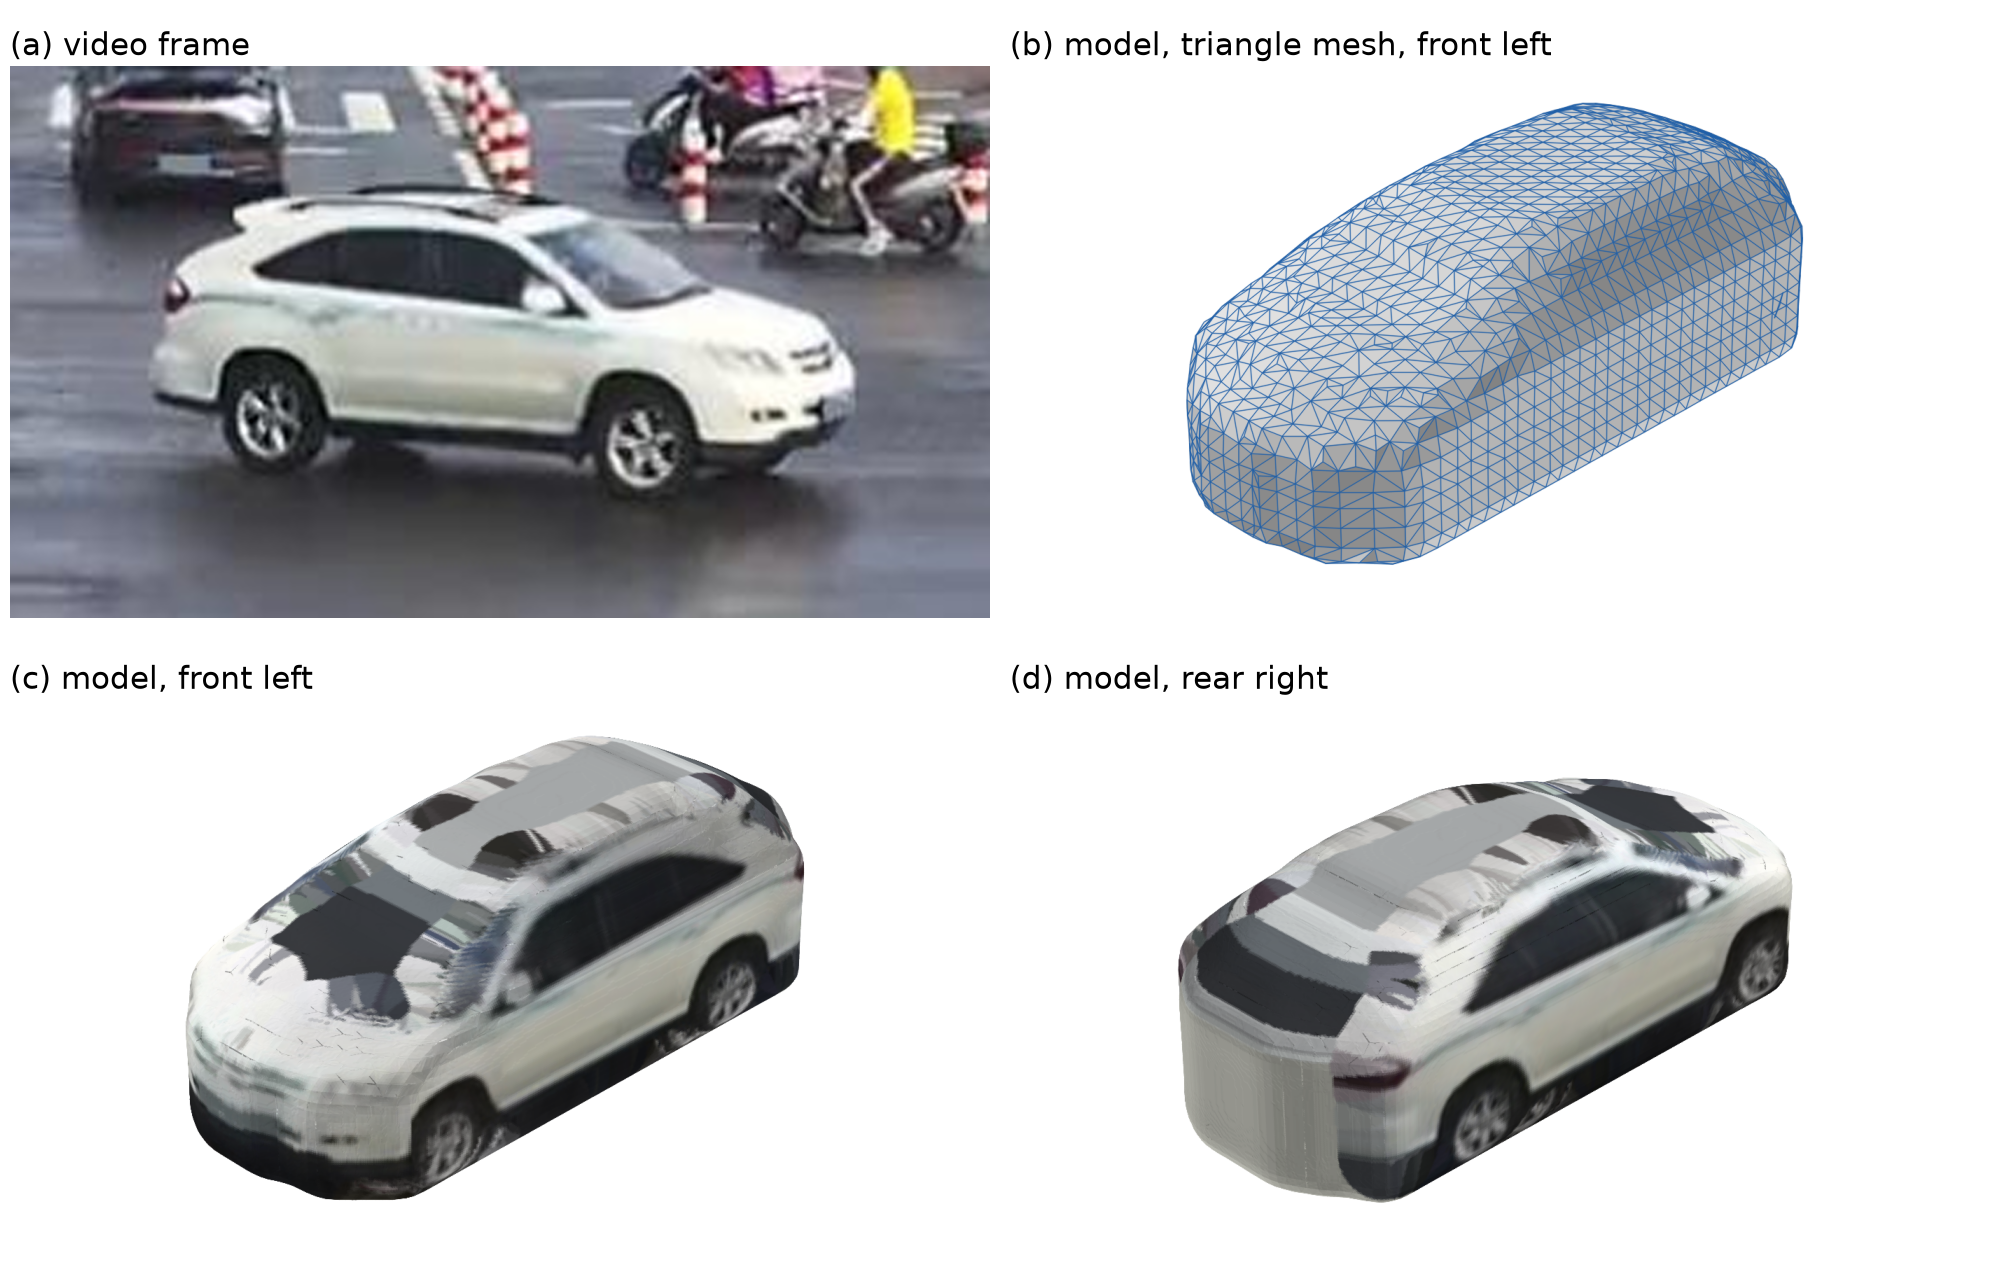
\includegraphics[width=\textwidth]{teaser.png}
\caption{One car of DAIR-V2X-C reconstructed end to end from the video of a single roadside camera, with the classical input (clip 114\_0, car 000046): (a) a frame of
the video; (b) the triangle mesh of the model fused over its 28 windows (shown coarsened); (c, d) the model with the
colours of the video, from the same viewpoint as (b) and from the opposite one, all from $30^\circ$ above the road; the right side, seen
in (d), is completed by symmetry. What no window saw takes a fill colour (the plain back,
Sect.~\ref{sec:completion}). Solid IoU 0.77 against the gap-closed LiDAR; 4.7~m long against the labelled 4.4~m.}
\label{fig:teaser}
\end{figure}

To our knowledge, no learning-free method recovers the full shape of moving vehicles from a single static camera.
Multibody structure from motion \cite{ozden2010} recovers sparse points of unknown scale per object; shape from
silhouettes across time \cite{cheung2005} needs the object to turn through a wide range of directions, which a car
passing an elevated camera does not; learned shape models \cite{kar2015,deepmanta} need a shape prior. The new elements
that make it possible here are:
\begin{enumerate}
\item \emph{triangulation with one unknown per vertex}: on a known road plane the motion of a car has three degrees of
  freedom per frame and each tracked vertex only its depth along its viewing ray; motion and depths are solved jointly
  in short windows under road contact and non-holonomic motion, and the one ambiguity a static camera leaves, a common
  scale about its centre, is fixed by the cuboid (Sect.~\ref{sec:window});
\item \emph{silhouettes from an elevated camera}: the visual hull of a passing car is biased along the viewing ray, and
  the top edge of each silhouette is the far edge of the roof, so the hull raises the near half of the roof by about
  $\tfrac{W}{2}\tan\epsilon$; the roof is therefore measured at that edge, and the length is measured only where the car
  is seen side-on (Sect.~\ref{sec:completion});
\item \emph{one rigid body per track}: all windows of a track share one pose per frame and are fused, with the
  symmetry plane, into a weighted-median height field: triangulated where the car is textured, the corrected hull
  where it is not (Sects.~\ref{sec:fusion}--\ref{sec:completion});
\item \emph{an unbiased LiDAR reference}: the raw accumulated LiDAR is strongly biased at long range (the labelled box
  itself scores \ClsALabRaw{} against it), and a gap-closed reference is proposed; against it, on \ClsTotalCars{} cars
  of two datasets and from the video alone, the shapes are level with the labelled boxes on the two development
  intersections and below them on the other clips (Sects.~\ref{sec:protocol}--\ref{sec:results}).
\end{enumerate}

% ------------------------------------------------------------------------------------------------------------------
\section{Related Work}

\paragraph{Monocular 3D detection.} Geometry-aware detectors fit a 3D box to a 2D detection
\cite{deep3dbox}; keypoint and centre-based networks regress boxes directly \cite{smoke,monodle,monoflex,gupnet,fcos3d};
others predict depth first \cite{pseudolidar,caddn} or lift image features to a bird's-eye view \cite{bevdet,bevdepth}.
For roadside cameras, BEVHeight \cite{bevheight} regresses the height above the ground instead of depth, which suits
the high viewpoint; Rope3D \cite{rope3d}, DAIR-V2X \cite{dairv2x} and V2X-Seq \cite{v2xseq} provide the benchmarks.
All of these are trained with 3D boxes and output boxes. Classical traffic-camera work calibrates the camera from
the vanishing points of the traffic \cite{dubska_diamond_space,dubska2015} and builds 3D bounding boxes of the vehicles
from them \cite{dubska2014,sochor}, segments and tracks vehicles from motion \cite{kanhere,moving_orig} and lifts 2D
detections to 3D with IPM \cite{mallot,lift,efficient_orig}; any of these can supply the input of our method.

\paragraph{Vehicle shape.} Learned category models fit a deformable car shape to a single image
\cite{kar2015,deepmanta,rcnn3d} or to stereo street scenes \cite{engelmann2016}; they need a shape prior learned from
CAD models or 3D annotations. Multibody structure from motion reconstructs several rigidly moving objects from point
tracks \cite{ozden2010}, and dense methods reconstruct dynamic scenes from two frames \cite{kumar2017}; bundle
adjustment \cite{bundleadj} refines both. Shape from silhouettes bounds an object by the intersection of its viewing
cones, the visual hull \cite{laurentini}, refined by photo-consistency in space carving \cite{spacecarving}. For one camera and a rigidly moving object,
shape from silhouette across time aligns the silhouettes of many frames by the object's estimated motion
\cite{cheung2005}; mirror symmetry completes the unseen half of an object seen from one side \cite{thrun2005}.

\paragraph{This work} differs from each of these in what it takes from a fixed, elevated camera. Unlike general
multibody structure from motion, it restricts the motion of the object to the road plane, so that every tracked vertex
has a single unknown and the surface is triangulated densely, with the scale from the cuboid. Unlike shape from
silhouettes across time, it does not need the object to turn: it corrects the bias of the hull along the viewing ray of
a high camera and takes the roof from the far edge of the silhouettes. Unlike learned shape models, it uses no shape
prior and no learned component.

% ------------------------------------------------------------------------------------------------------------------
\section{Setting}\label{sec:setting}

The camera is fixed and calibrated: a world point $\vect{X}$ projects to $\pi(\vect{X}) \sim \vect{K}(\vect{R}\vect{X} +
\vect{t})$. The world frame has the road as the plane $z = 0$; the road plane is fitted once, which amounts to measuring
the camera's height and tilt. A pixel $\vect{u}$ defines the ray
$\vect{X}(s) = \vect{C} + s\,\vect{d}(\vect{u})$ from the camera centre $\vect{C}$; its intersection with the road
is the inverse perspective mapping (IPM) \cite{mallot}. Cars move rigidly on the road plane: a point $\vect{X}$ of a
car moves from the reference frame to frame $j$ as
\begin{equation}
  \mathcal{M}_j(\vect{X}) = \begin{pmatrix} \vect{R}(\theta_j)(\vect{X}_{xy} - \vect{c}) + \vect{c} + \vect{t}_j \\ X_z \end{pmatrix},
  \label{eq:motion}
\end{equation}
with yaw change $\theta_j$, translation $\vect{t}_j \in \R^2$ and the car's centre $\vect{c}$ on the road.

% ------------------------------------------------------------------------------------------------------------------
\section{Method}

The method has five steps (Fig.~\ref{fig:pipeline}). The masks and cuboids of the moving objects come from any source (Sect.~\ref{sec:input}), for instance the
classical method of Sect.~\ref{sec:classical} (Fig.~\ref{fig:classical_steps}); the visible surface of every object is triangulated in
3D in short windows of the video (Sect.~\ref{sec:window}, Fig.~\ref{fig:steps} left); its orientation comes from
its motion (Sect.~\ref{sec:heading}, Fig.~\ref{fig:heading}); the windows of one object are solved together as one
rigid body (Sect.~\ref{sec:fusion}); and what the camera never sees is completed from symmetry, the masks and the
cuboid (Sect.~\ref{sec:completion}, Fig.~\ref{fig:steps}). Section~\ref{sec:system} collects the equations solved.

\begin{figure}[t]
\centering
\resizebox{\textwidth}{!}{%
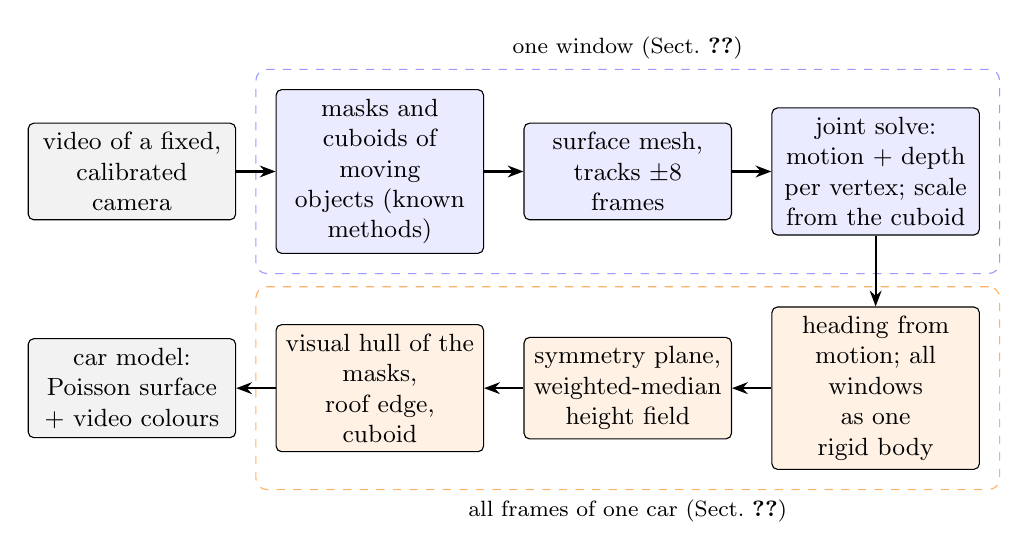
\begin{tikzpicture}[node distance=4mm and 5mm, every node/.style={font=\small},
  box/.style={draw, rounded corners=2pt, align=center, minimum height=11mm, text width=24mm, fill=#1},
  box/.default=white, arr/.style={-{Stealth[length=2mm]}, thick}]
  \node[box=gray!10] (video) {video of a fixed,\\ calibrated camera};
  \node[box=blue!8, right=of video] (seg) {masks and\\ cuboids of moving\\ objects (known\\ methods)};
  \node[box=blue!8, right=of seg] (mesh) {surface mesh,\\ tracks $\pm 8$ frames};
  \node[box=blue!8, right=of mesh] (solve) {joint solve:\\ motion + depth\\ per vertex; scale\\ from the cuboid};
  \node[box=orange!10, below=9mm of solve] (track) {heading from\\ motion; all windows\\ as one rigid body};
  \node[box=orange!10, left=of track] (sym) {symmetry plane,\\ weighted-median\\ height field};
  \node[box=orange!10, left=of sym] (hull) {visual hull of the\\ masks, roof edge,\\ cuboid};
  \node[box=gray!10, left=of hull] (model) {car model:\\ Poisson surface\\ + video colours};
  \draw[arr] (video) -- (seg); \draw[arr] (seg) -- (mesh); \draw[arr] (mesh) -- (solve);
  \draw[arr] (solve) -- (track); \draw[arr] (track) -- (sym); \draw[arr] (sym) -- (hull); \draw[arr] (hull) -- (model);
  \begin{scope}[on background layer]
    \node[draw=blue!40, dashed, rounded corners, fit=(seg)(mesh)(solve), inner sep=2.5mm, label={[font=\footnotesize]above:one window (Sect.~\ref{sec:window})}] {};
    \node[draw=orange!60, dashed, rounded corners, fit=(track)(sym)(hull), inner sep=2.5mm, label={[font=\footnotesize]below:all frames of one car (Sect.~\ref{sec:fusion})}] {};
  \end{scope}
\end{tikzpicture}}
\caption{The pipeline. Every window of up to $\pm 8$ frames is reconstructed on its own (blue); the windows of one object
are then fused over all frames that see it (orange). No step is learned.}
\label{fig:pipeline}
\end{figure}

\subsection{Masks and cuboids}\label{sec:input}

For every moving object the method takes its mask and its 3D cuboid (centre on the road, heading, length, width and
height) in the frames that see it, linked into tracks. Any source can supply them: the classical method of
Sect.~\ref{sec:classical}, or learned detectors and segmenters where better input is needed. All experiments of Sects.~\ref{sec:protocol}--\ref{sec:results} use the classical method; the labels of the
datasets serve only to pair a model with its LiDAR reference.

A window is built at every frame in which the object is neither occluded nor
cut by the image border. The method uses the cuboid's position and size; its heading serves
only to decide which triangulated points lie inside it (Sect.~\ref{sec:window}), and the orientation of the object
comes from its motion (Sect.~\ref{sec:heading}).

\subsection{A classical input}\label{sec:classical}

The classical input is obtained from the video alone (Fig.~\ref{fig:classical_steps}). It follows the moving-object
detection and segmentation of \cite{moving_orig}, segments of coherent optical flow merged into objects while they fit
an object type, with the lifting replaced by the tangent construction of \cite{dubska2014} and a track stage added; it
runs at half resolution.

\begin{figure}[!htbp]
\centering
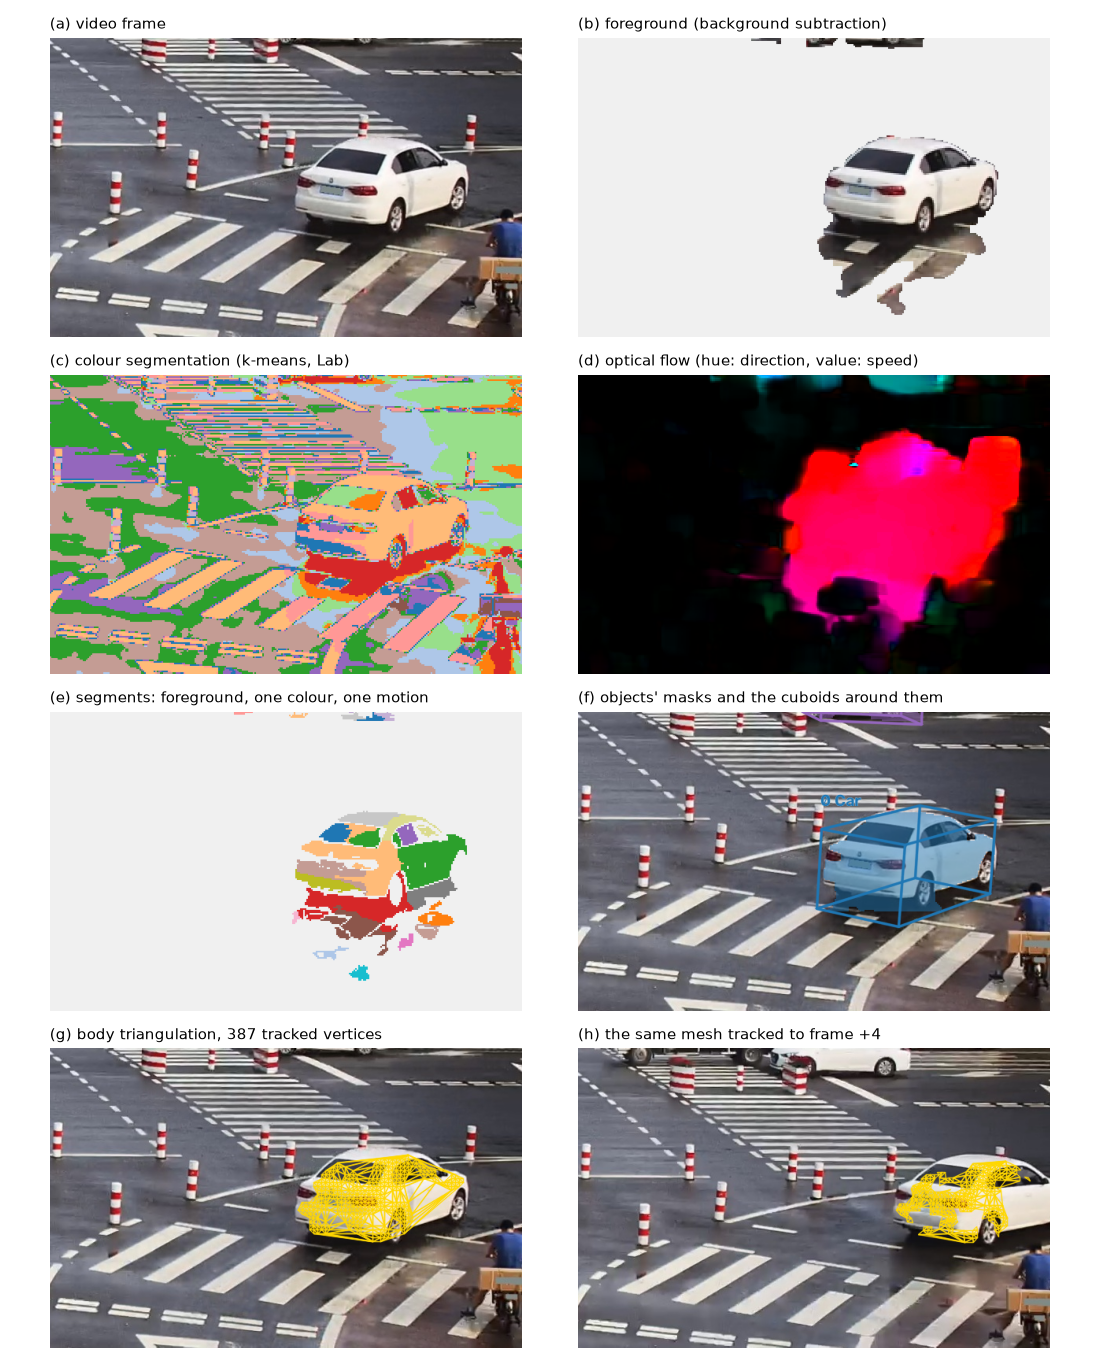
\includegraphics[width=\textwidth]{classical_steps.png}
\caption{The classical input around one car of intersection A (frame 010871): (a) the frame; (b) the foreground of
the background subtraction, with the car's shadow on the wet road; (c) the optical flow, its direction as hue and its
speed as value; (d) the segments, foreground lying inside one colour and one motion (the shadow forms segments of its
own); (e) the object's mask, merged from the car's segments without the shadow, its silhouette (white) and the cuboid
built around it: the tangents from the vanishing points of the direction of motion (red), the lateral (green) and the
vertical direction (blue) touch the box along its edges (dots), and the box's size is measured; (f) the body
triangulation of its window (Sect.~\ref{sec:window}): vertices on a grid inside the eroded mask, tracked through up to $\pm 8$ frames, triangulated by Delaunay.}
\label{fig:classical_steps}
\end{figure}

\paragraph{Segments.} Three segmentations of every frame are intersected. The foreground comes from a background
subtractor that keeps for every pixel samples of its colour and of its local binary patterns and adapts its
thresholds by feedback (GSOC, after SuBSENSE \cite{subsense}); the colour segmentation is a $k$-means quantisation of
the frame's Lab colours; and, as in \cite{moving_orig}, the dense optical flow \cite{farneback} is coded in HSV, its
direction as hue and its magnitude as value, and quantised by $k$-means. A segment is a connected region that is
foreground and lies wholly inside one colour segment and one moving flow segment; a segment much smaller than a car
at its distance joins its largest neighbour that moves alike.

\paragraph{Objects and cuboids.} Starting from the largest, neighbouring segments that move alike are merged into an
object one at a time, each time the one whose merge fits an object type best, and the best of these merges is kept
\cite{moving_orig}; a large segment of another colour that widens the object is another car's body and is not merged.
The cuboid of an object is built around its silhouette (Fig.~\ref{fig:classical_steps}e). Its axes are the direction
of motion, from the optical flow on the road, the lateral and the vertical direction, and each has a vanishing point;
the two tangents from a vanishing point to the silhouette are the images of two planes through the camera centre that
touch the box along an edge \cite{dubska2014}. With the calibrated camera each tangency is a linear equation in the
box's extents along the two horizontal axes and its height: six tangents for five unknowns, solved by least squares,
with the edge each tangent touches assigned from the current box and the solve repeated. The size is measured, and
the object's type is the one whose average size it deviates least from; that deviation also decides the merging. (The
lifting of \cite{moving_orig}, which fixes the type's length and inscribes the footprint in the inverse perspective
quadrangle of the 2D box, leaves the width undetermined for a car that crosses the view far away.) On the wet road a
car's mirror image is cut off at the contact line, below which the image is the car mirrored and blurred, and the
tangents along a nearer object are left out.

\paragraph{Tracks.} The objects are linked in the image, each track's 2D box moved by its optical flow. Per track, the
heading is the flow's direction of motion averaged over the neighbouring frames, and the size is the median of the
measured sizes. A track is predicted along its smoothed path, also a few frames beyond its ends: an object whose box
holds the predictions of two tracks, two cars that touch in some frames, is divided between them, and a frame without
an object of the track gets its prediction.

\subsection{Triangulation of one window}\label{sec:window}

\paragraph{The surface and its mesh.} The mask of the reference frame, slightly eroded so that no vertex lies on its
outline, receives a regular grid of vertices, triangulated by Delaunay. The window is at most $\pm 8$ frames around the reference frame; for a fast or near object it is shortened to the frames in which the object moves at most 100~px in the image from the reference, but not below $\pm 3$ frames . Every vertex is tracked through the window with pyramidal Lucas--Kanade \cite{lucas_kanade} and a forward--backward check, and kept if it is
followed in most of them.

\paragraph{Joint solve.} The unknowns are the motion $\vect{m}_j = (\theta_j, \vect{t}_j)$ of the car in every frame
of the window ($\vect{m}_r = 0$ in the reference frame $r$) and the depth $s_i$ of every vertex along its reference
ray, $\vect{X}_i = \vect{C} + s_i \vect{d}_i$. They minimise
\begin{align}
  E = &\sum_{i,j} \big\| \pi_j\big(\mathcal{M}_j(\vect{X}_i)\big) - \vect{u}_{ij} \big\|^2
      + \lambda \sum_{(a,b)} w_{ab} \|\vect{n}_a - \vect{n}_b\|^2
      + W_a \sum_{i \in \mathcal{L}} X_{i,z}^2 \nonumber\\
      &+ W_m \sum_j \|\vect{m}_{j-1} - 2\vect{m}_j + \vect{m}_{j+1}\|^2_{\Sigma}
      + W_h \sum_j \big( \vect{e}_\perp \cdot \vect{R}(-\bar\theta_j)(\vect{t}_{j+1} - \vect{t}_j) \big)^2 ,
  \label{eq:energy}
\end{align}
with every squared residual $r^2$ entering through the robust soft-$\ell_1$ loss $\rho(r^2) = 2(\sqrt{1 + r^2} - 1)$,
which grows only linearly for large residuals. The first term is the reprojection error of the tracked vertices. The
second makes the normals $\vect{n}_a, \vect{n}_b$ of triangles sharing an edge agree, with a lower weight $w_{ab}$
across a colour edge, so that panels stay smooth and creases follow paint and trim lines. The third puts the tyres on
the road: $\mathcal{L}$ holds the vertices on the mask's bottom row, where the tyres touch the road; vertices below
that row belong to the mirror image on a wet road and are kept below the road. The fourth is temporal smoothness of
the motion, in the norm $\|\vect{m}\|^2_{\Sigma} = \vect{m}^\top \Sigma^{-1} \vect{m}$, whose $\Sigma$ weighs yaw against
translation; the fifth forbids a sideways step: a
car moves along its heading ($\vect{e}_\perp$ is the lateral normal of the initial direction of travel, $\bar\theta_j$
the mean yaw of the step). Both motion priors are divided by the length of the path, so that they do not favour a smaller
copy of the car closer to the camera, which would move less. Every other vertex is bounded between the road and the height of a car.

The motion is initialised by a RANSAC Procrustes fit \cite{fischler_bolles_ransac} of the IPM points of the lowest
vertices, frame to frame, smoothed by a quadratic in time; the yaw change follows the direction of the path. The
depths start at the intersection of each vertex's rays under that motion. After the solve, vertices with a large
residual --- background dragged along by the tracker at the outline, or another car --- are removed and the solve is
repeated.

\paragraph{Scale from the cuboid.} A fixed camera sees a window and the same window scaled about the camera centre
identically in every frame, since the motion and the depths scale alike: the images fix the shape, not the scale. The
tyres on the road fix it, but at 60--70~m a pixel of the contact row moves the object by decimetres. The window is
therefore scaled about the camera centre by the factor that puts the most vertices inside its cuboid, and vertices
far outside the cuboid, or outside the mask in the reference frame, are dropped as depth outliers along the ray. The
cuboid fixes where the object is and how large; its shape still comes from the triangulation.

\subsection{Orientation from motion}\label{sec:heading}

\begin{figure}[t]
\centering
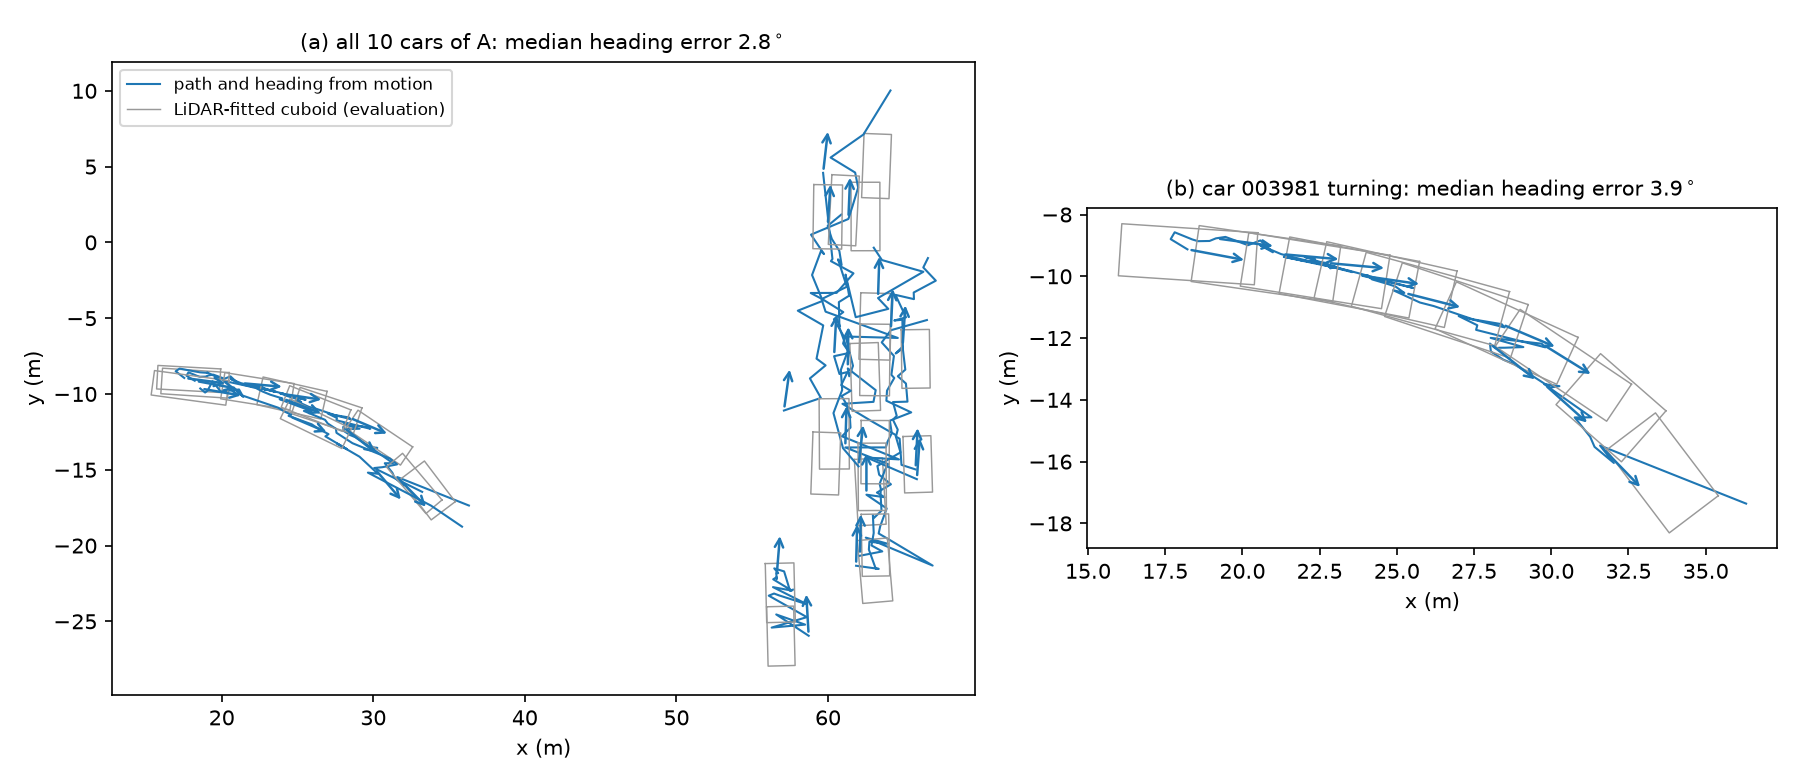
\includegraphics[width=\textwidth]{heading.png}
\caption{Orientation from motion, intersection A. (a) The path of every car and its heading from the track solve
(blue arrows), with the labelled cuboids (grey, evaluation only); (b) a turning car up close. The
heading follows the direction of travel through the turn; median error against the labelled yaw $\ClsAHeading^\circ$ over the \ClsACars{} cars of A.}
\label{fig:heading}
\end{figure}

\paragraph{Heading.} The orientation of a car is never fitted to its shape, nor taken from its cuboid; it comes from
its motion, as a car drives along its heading. In a window, the yaw changes $\theta_j$ are unknowns of Eq.~(\ref{eq:energy}), started from a RANSAC
Procrustes fit of the lowest vertices; the window's velocity is the solved translation per frame. Over the track,
these velocities are smoothed by a quadratic in time, and the heading of each window is the direction of the smoothed
velocity,
\begin{equation}
  \psi_w = \operatorname{atan2}\big(\bar v_{w,y},\, \bar v_{w,x}\big),
  \label{eq:heading}
\end{equation}
for the smoothed velocity $\bar{\vect{v}}_w$ at the window's reference frame. This heading starts the track solve,
whose pose $\vect{Q}_g = (\phi_g, \vect{p}_g)$ then gives the car's heading $\phi_g$ in every frame; the last term of
Eq.~(\ref{eq:track}) keeps it along the direction of travel.

\paragraph{The car's box.} The car frame has its $x$ axis along $\phi_g$, and the model is built in it, so the car's
bounding box is aligned with the heading: its length and width are the extents of the occupied height-field columns
along $x$ and $y$, its height a high percentile of the column heights. A car that turns is therefore boxed along its
momentary direction of travel. Figure~\ref{fig:heading} shows the paths and headings of the cars of A; the heading
errors of all sets are given in Sect.~\ref{sec:results}.

\subsection{One rigid body per track}\label{sec:fusion}

\paragraph{Tracks.} The windows of one object are linked by the track identities of the input. Tracks of fewer than
five windows are dropped.

\paragraph{One rigid car per track.} Each window has solved its own motion, so two windows of the same car disagree
on where the car is when they overlap in time. We therefore solve all windows of a track together, as rigid structure
from motion of one moving object \cite{ozden2010}: one planar pose $\vect{Q}_g = (\phi_g, \vect{p}_g)$ of the car per
frame $g$, shared by every window that sees frame $g$, and the depths of all windows' vertices. A vertex of window $w$,
a point $\vect{X}$ in the world at the window's reference frame $r_w$, is at
$\vect{X}^{(g)} = \big(\vect{R}(\phi_g - \phi_{r_w})(\vect{X}_{xy} - \vect{p}_{r_w}) + \vect{p}_g,\; X_z\big)$ in
frame $g$. The energy is that of Eq.~(\ref{eq:energy}) summed over the windows, with the motion terms on the shared
poses of the whole track:
\begin{align}
  E_{\text{track}} = &\sum_{w} \Big[ \sum_{i \in w} \sum_{g} \big\| \pi_g\big(\vect{X}_i^{(g)}\big) - \vect{u}_{ig} \big\|^2 \nonumber\\
    &\quad + \lambda \sum_{(a,b) \in w} w_{ab} \|\vect{n}_a - \vect{n}_b\|^2
      + W_a \sum_{i \in \mathcal{L}_w} X_{i,z}^2 \Big] \nonumber\\
    &+ W_m \sum_g \big\|\vect{Q}_{g-1} - 2\vect{Q}_g + \vect{Q}_{g+1}\big\|^2_{\Sigma} \nonumber\\
    &+ W_h \sum_g \big( \vect{e}_\perp(\bar\phi_g) \cdot (\vect{p}_{g+1} - \vect{p}_g) \big)^2 ,
  \label{eq:track}
\end{align}
over the poses $\vect{Q}_g$ and the depths $s_i$ of all vertices ($\vect{X}_i = \vect{C} + s_i \vect{d}_i$ along the
reference ray of its window), where $\vect{e}_\perp(\phi) = (-\sin\phi, \cos\phi)$ is the lateral normal of the
heading $\phi$ and $\bar\phi_g$ the mean heading of the step, and with the weights and bounds of the windows. As in Eq.~(\ref{eq:energy}), every squared residual enters
through the soft-$\ell_1$ loss $\rho$. One pose is held fixed,
which removes the gauge freedom (a common planar motion of all poses and points). The solve starts from a chain: the middle window's pose comes from the
smoothed path of the track, and each window places the reference frame of its neighbour through its own solved
motion, so that the start agrees with every window's points. The vertices on the outline of a window's triangulation
are left out: the tracker follows the moving edge of the car's mask there, not a point of its surface, and with them
the track solve stretches the cars. Every window then enters the car frame ($x$ forward, $y$ left, $z$ up) through the
shared pose of its reference frame, with no further alignment.

\subsection{Completion of what the camera does not see}\label{sec:completion}

\begin{figure}[t]
\centering
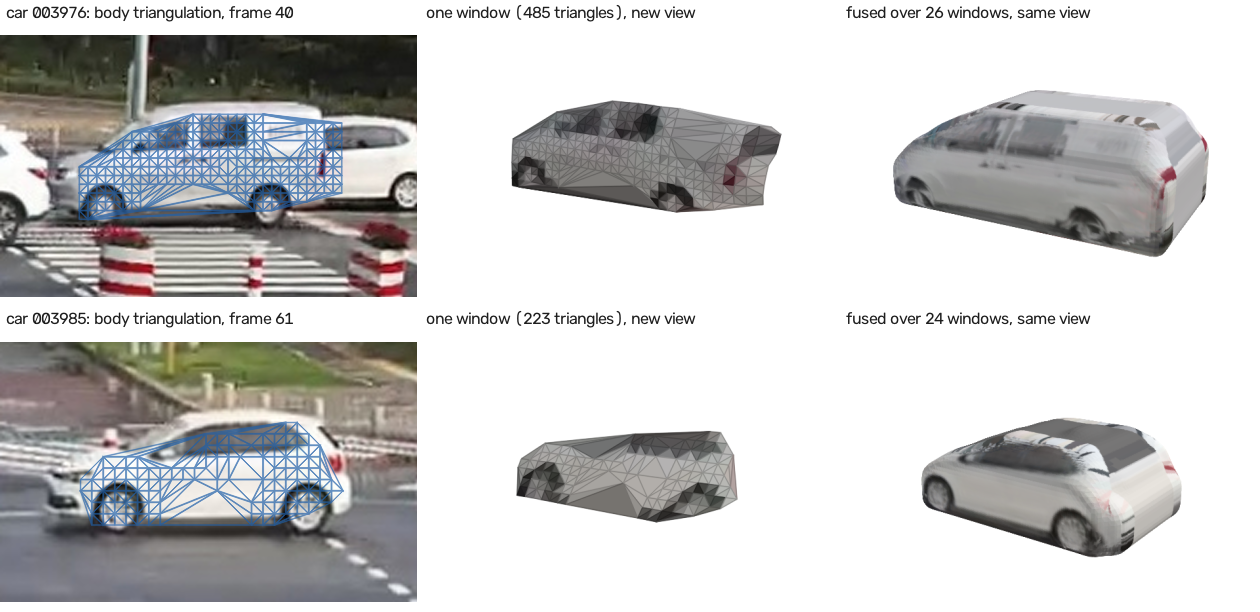
\includegraphics[width=\textwidth]{method_steps.png}
\caption{From triangulation to model, two cars of intersection A, from the classical input. Left: the body triangulation in one frame.
Middle: the same triangles in 3D after the window's joint solve, from a new viewpoint --- one window is noisy along
the viewing rays. Right: the model fused over all windows of the car (one rigid car, symmetry, weighted-median height
field, cabin from silhouettes, Poisson surface, video colours), from the same viewpoint.}
\label{fig:steps}
\end{figure}

\paragraph{Symmetry.} The symmetry plane $y = y_0$ maximises the share of points whose mirror image has a close
neighbour \cite{mitra2006}; the points are re-centred on it and used together with their mirror images, which gives
the unseen side of the car. Points beyond the width of the widest car are dropped.

\paragraph{Height field.} In every column of the car frame each window contributes the height of its highest point.
The model height is the median over the windows that saw the column, weighted by each window's reprojection error,
and a column must be seen by several windows. Columns with few points compared with the densest column of the same
cross-section are dropped: the true surface collects points from every window, the along-ray depth noise spreads them
thin. A median filter and the largest connected component finish the field.

\paragraph{Cabin from the masks.} The triangulated field covers the textured surface; the glass and the roof are often too
dark or too uniform to track. The silhouette of the object in every frame is its mask; the masks of the frames in
which the object is unoccluded and inside the image carve. Voxels are kept if they, and their mirror images, project
inside the mask in at least 75\,\% of the frames that see them (a visual hull \cite{laurentini} with a soft vote: the masks and poses are not exact); the top of the kept voxels is
the cabin field, and the model is the higher of the triangulated and cabin fields. A high camera sees a car from
nearly the same direction in all frames, so the cone of one silhouette is long along the viewing ray and rises toward
the camera; the hull is therefore capped a little above the cuboid's height. For near objects the silhouettes alone
are used.

\paragraph{Roof from the far edge.} The camera is above the car, so the top edge of a silhouette is the \emph{far}
edge of the roof, and the visual hull lets the near half of the roof rise by about $\tfrac{W}{2}\tan\epsilon$ above
it, for the width $W$ and the camera's elevation angle $\epsilon$. The roof height $r(x)$ at each position $x$ along
the car is therefore measured where it is seen: in every frame, a vertical segment at $x$ on the far side of the car
is projected, and $r(x)$ is the height at which it leaves the mask through its top edge. The median over the frames
caps the height field. This holds where the viewing ray runs along the car --- a car seen only from behind, whose hull
overshoots by about $\tfrac{L}{2}\tan\epsilon$ --- and the cap is applied only to cars never seen side-on. Seen
side-on, the top edge of the mask is the crown of the rounded roof rather than its far edge, and the cap would lower
the car.

\paragraph{Body type and width.} The side profile of the car's silhouette in its most side-on windows gives
scale-free features (length to height, share of the length under the roof, height of the front and rear) and a type
by fixed rules: sedan, hatchback, SUV or van. For a car seen from the side the width lies nearly along the viewing
ray, where a single camera measures it worst; the width is therefore bounded about the symmetry plane by the type's
typical width with its mirrors, which the LiDAR sees and a cuboid fitted to the body leaves out. The cabin is narrower than the body, and its near upper edge is never seen against the background; across the car the field is therefore capped by a fixed profile, a roof over 72\,\% of the width and sides that lean inward above the belt line at 62\,\% of the height. 

\paragraph{Length.} The length is measured only where the car is seen side-on, i.e.\ where the viewing ray crosses the car at a large angle. A car seen
side-on in fewer than two windows --- most often a car seen only from behind --- has a length and a profile the video
never measured, only a silhouette cone that is long along the ray. It is completed from its cuboid: the footprint of
the cuboid's length and width about the middle of the cone and the symmetry plane, and the profile of its body type
scaled to the cuboid's height, a box up to the shoulder line and a cabin box on top with a sloping windshield and rear
window. This is completion, not measurement. Cars measured side-on, vans included, keep their own length and shape.

\paragraph{Surface.} The height field is regularised between its raw surface and a convex hull: every
cross-section of the car becomes its upper concave envelope, which fills notches and holes in the roof, while along
the car narrow spikes and thin sheets are removed and narrow dips are filled (grey-scale opening and closing), so that
the steps from bonnet to windshield to roof survive. The surface of the regularised field (marching cubes
\cite{marchingcubes}) is finally replaced by its Poisson surface \cite{kazhdan2006}, which removes the staircase of
the columns; this changes the shown model, not the height field that is evaluated.

\paragraph{Colour.} For the figures the Poisson
surface is subdivided to about the size of a camera pixel on the car and coloured there. Every vertex takes the
original pixels of the views that see it best --- facing it and near --- where it lies inside the car's silhouette and
is not hidden by another part of the model; of these the medoid colour is kept, so that one view whose pose is a
little off is outvoted. Before sampling a view, the model's projected outline is shifted onto that window's
silhouette: the windows at the ends of a track are often off by tens of pixels, and without this the glass lands on
the bonnet. A vertex and its mirror image take the better seen of the two. A vertex no window sees takes the colour of
a nearby seen vertex; farther from one, below the belt line one body colour, and above it the median colour of the
seen vertices at the same height --- glass at cabin height --- except that an upward-facing vertex, on the bonnet or the
roof, takes the colour of the seen upward-facing ones, the paint.

\subsection{The system of equations}\label{sec:system}

For one object, with masks $M_g$ and cuboids $B_g$ in its frames $g$, the method solves in turn:
\begin{enumerate}
\item \emph{each window} $w$ (reference frame $r_w$, frames within $r_w \pm 8$): Eq.~(\ref{eq:energy}) over the motion
  $\vect{m}_j$ and the depths $s_i$ of the vertices, with the vertices bounded between the road and the height of a
  car (below the road for the mirror image on a wet road), started from the IPM of the lowest vertices;
\item \emph{its scale}: $\sigma_w = \arg\max_{\sigma} \big|\{ i : \vect{C} + \sigma (\vect{X}_i - \vect{C})
  \in B_{r_w} \oplus \delta \}\big|$ for a small margin $\delta$, every vertex then moved to
  $\vect{C} + \sigma_w (\vect{X}_i - \vect{C})$, and the vertices far outside $B_{r_w}$, or outside $M_{r_w}$,
  dropped;
\item \emph{the heading} of each window from the motion, Eq.~(\ref{eq:heading});
\item \emph{the track}: Eq.~(\ref{eq:track}) over the poses $\vect{Q}_g$ and all depths $s_i$, started from the chain
  of windows and the headings;
\item \emph{the shape} in the car frame: the height field $H$, the weighted median over the windows of the highest
  point per column, mirrored about the symmetry plane; the cabin $H_c$, the top of the voxels that project into the
  masks of most frames, mirrored, capped near the cuboid's height; the model $\max(H, H_c)$,
  capped by the roof line $r(x)$ and completed from the cuboid where the car was never seen side-on, and bounded by the
  width.
\end{enumerate}
Steps 1 and 4 are non-linear least squares; every residual enters through the soft-$\ell_1$ loss, and they are solved
by a trust-region method with bounds and a sparse finite-difference Jacobian, stopped after a fixed number of evaluations (60 for a window, 40 for a track). Steps 2, 3 and 5 are closed-form or a one-dimensional
search. The weights and thresholds were set once on intersection A and are the same for every object and dataset.

% ------------------------------------------------------------------------------------------------------------------
\section{Evaluation Protocol}\label{sec:protocol}

\paragraph{Datasets.} \emph{Intersection A} is the infrastructure side of the V2X-Seq-SPD example \cite{v2xseq}
(sequence 0058, 251 frames at 10~Hz, $1920 \times 1080$, camera 8.45~m above the road and tilted $15^\circ$ down,
wet road). \emph{Intersection B} is the infrastructure side of the DAIR-V2X-C example \cite{dairv2x} (84 frames at
12.5~Hz, camera 8.96~m above the road, dry road); its labels have no track identities, so we link the labelled boxes from frame to frame. Three further clips of DAIR-V2X-C (114, 105 and 52) and four further sequences of V2X-Seq-SPD (0002, 0054, 0059 and 0077) complete the evaluation; frames missing from a recording are skipped and the motion is measured per time slot.

\paragraph{Tuning.} The parameters of the reconstruction were chosen on intersection A, during development and with
masks and cuboids more precise than the classical ones, derived from the labels and the LiDAR. Three design choices
also looked at B and at clips of the two datasets: the length cap only for cars never seen side-on, rather than for
every car; the soft hull vote (Sect.~\ref{sec:completion}); and the joint solve of a track. Every result reported
here uses the classical input with no parameter changed, but no set is a clean hold-out of the design.

\paragraph{LiDAR reference.} For each labelled car the LiDAR points inside its box are collected over its whole track
in the box frame, mirrored about the box's vertical centre plane along its heading and turned into a height field of
5~cm columns. This \emph{symmetry-completed} reference fills the side the LiDAR did not see; it favours symmetric
shapes, but our models and the labelled boxes are both symmetric, so it favours neither over the other. A car is
evaluated when its reference holds enough points and one of our tracks is matched to it.

\paragraph{The reference is biased.} At 60~m a LiDAR scan is sparse: the accumulated points leave gaps between scan
lines on the roof and the bonnet, and these gaps are counted as empty space. Scored against the raw field, the
\emph{labelled box itself} reaches a mean solid IoU of only \ClsALabRaw{} on intersection A --- about what our models
score --- so the raw reference cannot rank methods near the top. We close the gaps by a grey-scale closing of the
height field with a radius of 15~cm, which fills gaps between returns but does not extend the outline; against the
gap-closed field the labelled box scores \ClsALab{} on A and \ClsBLab{} on B. We report both references.
Figure~\ref{fig:lidar} shows the effect for two cars.

\begin{figure}[t]
\centering
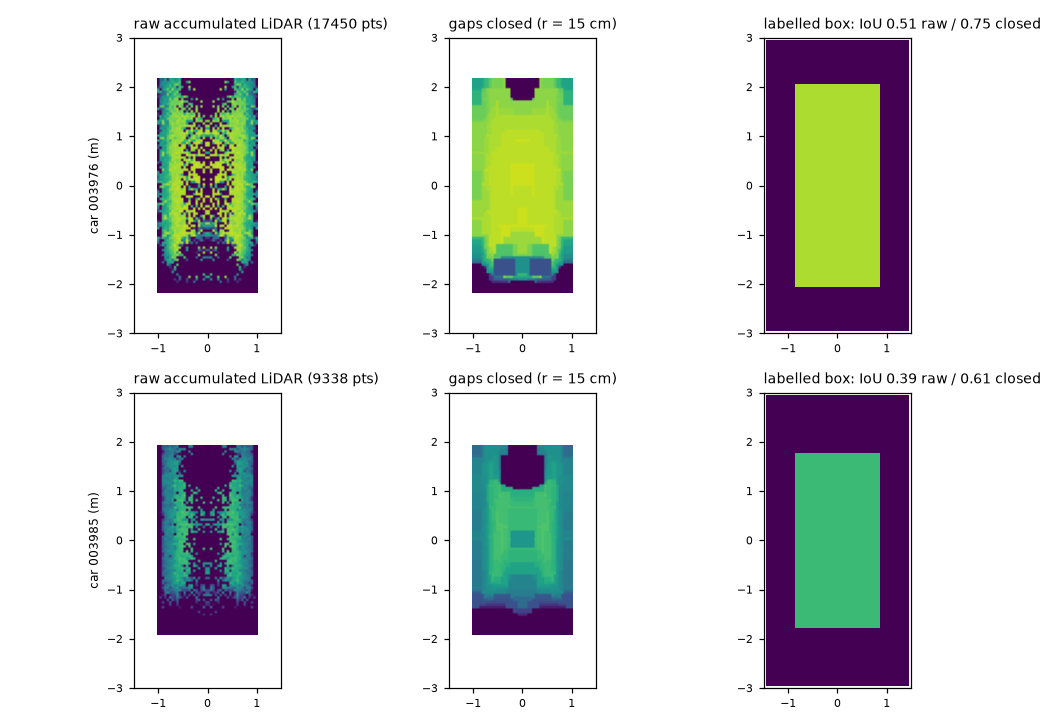
\includegraphics[width=0.85\textwidth]{lidar_reference.png}
\caption{The LiDAR reference of two cars of intersection A in the car frame (colour: height, 0--2~m). The raw
accumulated field has gaps between the scan lines (left); closed with a radius of 15~cm it keeps the outline
(middle). The labelled box (right) scores far lower against the raw field than against the gap-closed one.}
\label{fig:lidar}
\end{figure}

\paragraph{Metrics.} Both height fields are centred on their footprints and compared with both headings. The
\emph{solid IoU} is $\sum \min(H, L) / \sum \max(H, L)$ over all columns, for our height field $H$ and the reference
$L$, on a grid that covers both, so that a model longer or wider than the car is penalised; the \emph{footprint IoU}
compares the occupied columns; the \emph{height error} is the median $|H - L|$ over columns occupied in both. Length, width and height are compared with the labelled box. As a check that the closing does not favour
smooth models, the \emph{scanned IoU} leaves out only the reference volume the closing invented (columns without a
return in the raw field), keeping every other column, so that a model sticking out of the car still counts. Paired
differences between our models and the labelled boxes on the same cars are given with 95\,\% bootstrap intervals
(5000 resamples); a label our tracker split into two track fragments keeps the longer one.

% ------------------------------------------------------------------------------------------------------------------
\section{Results}\label{sec:results}

\begin{table}[t]
\centering
\caption{Car models from the video alone against their accumulated LiDAR: mean solid IoU against the gap-closed reference, on intersections A and B, three clips of DAIR-V2X-C and four sequences of V2X-Seq-SPD. The labelled box, a box of our own estimated size, the input cuboid of the classical method and the best single window are scored in the same way; the last two columns pair our models with the labelled box and with their input cuboid on the same cars (mean difference, 95\,\% bootstrap interval, 5000 resamples).}
\label{tab:main}
\setlength{\tabcolsep}{0.8pt}
\footnotesize
\begin{tabular}{lrccccccc}
\toprule
 & cars & ours & labelled & box of & input & single & ours $-$ labelled & ours $-$ input \\
 & & & box & our size & cuboid & window & & \\
\midrule
A & 8 & 0.589 & 0.572 & 0.607 & 0.552 & 0.275 & $+0.017$ $[-0.071, +0.093]$ & $+0.037$ $[-0.069, +0.130]$ \\
B & 9 & 0.507 & 0.508 & 0.484 & 0.504 & 0.401 & $-0.001$ $[-0.080, +0.058]$ & $+0.002$ $[-0.063, +0.055]$ \\
DAIR-V2X-C & 24 & 0.584 & 0.637 & 0.615 & 0.599 & 0.223 & $-0.053$ $[-0.103, -0.003]$ & $-0.015$ $[-0.066, +0.037]$ \\
V2X-Seq-SPD & 30 & 0.554 & 0.649 & 0.587 & 0.617 & 0.292 & $-0.095$ $[-0.158, -0.039]$ & $-0.062$ $[-0.120, -0.007]$ \\
\bottomrule
\end{tabular}
\end{table}

\paragraph{Intersection A (tuning set).} Table~\ref{tab:main} compares the models with four references scored in
the same way: the labelled box, a box of our own estimated length, width and height, the cuboid the classical method
gave as input, and the best single window without averaging and symmetry. A car is paired with its label over its
whole track. Of the 24 moving cars of A with a LiDAR reference, \ClsACars{} get a model: the classical input misses
or merges the others (Table~\ref{tab:classical}). Against the gap-closed reference the models reach \ClsAOurs{},
against \ClsALab{} for the labelled boxes and \ClsAInput{} for their input cuboids; with \ClsACars{} cars the
intervals of both differences include zero. A box of the models' own size scores \ClsAOwn{}
(ours minus that box: \ClsADOwn{}): on A the shape does not add to its dimensions. Against the raw reference the
models reach \ClsAOursRaw{} and the labelled boxes \ClsALabRaw{}. A single window reaches only \ClsASingle{}
(\ClsADSingle{}); the gain comes from fusing the video (Fig.~\ref{fig:steps}). The length is off by a mean of
\ClsALerr{}~m, the width by \ClsAWerr{}~m and the height by \ClsAHerr{}~m against the labelled box, and the height
field by \ClsAFieldErr{}~cm against the LiDAR. About a third of the occupied columns of the gap-closed reference were
added by the closing itself (mean filled share \ClsAFilled{} on A); scored on all columns except that invented
volume, the pair barely changes: a scanned IoU of \ClsAScanned{} against \ClsALabScanned{} for the labelled box.
Figure~\ref{fig:cars} shows four of the models up close, drawn into their frames, with their LiDAR.

\paragraph{Intersection B.} The same method reaches \ClsBOurs{} against \ClsBLab{} for the labelled boxes and
\ClsBInput{} for the input cuboids (Table~\ref{tab:main}), for \ClsBCars{} of the 15 cars with a LiDAR reference. B
is harder than A: all cars drive away from the camera and are seen only from behind. The textured part is then the
rear, whose depth is measured along the viewing ray, and the silhouette cone is long in the same direction. No
window of them is side-on, so their length comes from the cuboid, and their roof from the far edge of the masks. The
models are ahead of a box of their own size, within the interval (\ClsBDOwn{}), and the height field is off by
\ClsBFieldErr{}~cm.

\begin{table}[t]
\centering
\caption{The same evaluation per clip, no parameter changed: mean solid IoU of our models and of the labelled boxes against the raw and the gap-closed LiDAR, of the input cuboids against the gap-closed one, and the median error of the car's centre along the viewing ray.}
\label{tab:clips}
\footnotesize
\begin{tabular}{llrcccccc}
\toprule
 & & & \multicolumn{2}{c}{raw LiDAR} & \multicolumn{3}{c}{closed LiDAR} & along \\
\cmidrule(lr){4-5}\cmidrule(lr){6-8}
 & clip & cars & ours & box & ours & box & input & ray (m) \\
\midrule
intersection A & V2X-Seq-SPD 0058 & 8 & 0.414 & 0.374 & 0.589 & 0.572 & 0.552 & 0.82 \\
intersection B & DAIR-V2X-C example & 9 & 0.357 & 0.322 & 0.507 & 0.508 & 0.504 & 2.22 \\
DAIR-V2X-C & clip 114 & 4 & 0.596 & 0.501 & 0.702 & 0.633 & 0.599 & 1.96 \\
 & clip 105 & 8 & 0.412 & 0.416 & 0.531 & 0.547 & 0.491 & 2.17 \\
 & clip 52 & 12 & 0.596 & 0.635 & 0.580 & 0.697 & 0.671 & 2.21 \\
V2X-Seq-SPD & seq. 0054 & 9 & 0.481 & 0.529 & 0.618 & 0.687 & 0.651 & 0.80 \\
 & seq. 0059 & 8 & 0.375 & 0.393 & 0.513 & 0.531 & 0.482 & 0.42 \\
 & seq. 0077 & 2 & 0.454 & 0.405 & 0.679 & 0.543 & 0.598 & 1.75 \\
 & seq. 0002 & 11 & 0.559 & 0.702 & 0.510 & 0.724 & 0.690 & 2.33 \\
\bottomrule
\end{tabular}
\end{table}

\paragraph{Further clips of the two datasets.} Unchanged, the chain was run on three clips of DAIR-V2X-C and four
sequences of V2X-Seq-SPD (Table~\ref{tab:clips}). The \ClsDCars{} cars of DAIR-V2X-C reach \ClsDOurs{} against
\ClsDLab{} for the labelled boxes, the \ClsSCars{} cars of V2X-Seq-SPD \ClsSOurs{} against \ClsSLab{}: the models
are below the labelled boxes on both (\ClsDDLab{} and \ClsSDLab{}). Against their own input cuboids they are level
on DAIR-V2X-C (\ClsDDInput{}) and below on V2X-Seq-SPD (\ClsSDInput{}). They are ahead of the labelled box in two
of the seven clips, 114 and 0077, with four and two cars; the largest deficits are in clip 52 and sequence 0002,
the two with the most scored cars. Figure~\ref{fig:large} shows eight car models of both datasets
next to the cars in the video.

\paragraph{Position and heading.} The shapes are compared in the car's own frame; its position is compared with the
label. On A the car's centre is off by a median of \ClsAAlong{}~m along the viewing ray and \ClsAAcross{}~m across
it, on the clips of DAIR-V2X-C and V2X-Seq-SPD by \ClsDAlong{}~m and \ClsSAlong{}~m along the ray. On B it is off
by \ClsBAlong{}~m along the ray; there the camera and the LiDAR of the dataset are not synchronised: the model
stands at the camera's time, the label at the LiDAR's, and a car at traffic speed travels a few metres between the
two clocks, along the direction of travel, which on B is the viewing ray. A car is therefore paired with its label
over its whole track, not by its position in a single frame. The heading from the motion is accurate: against the
labelled yaw (modulo $180^\circ$, per car the median over its windows) the median error is \ClsAHeading$^\circ$ on A
and \ClsBHeading$^\circ$ on B, \ClsDHeading$^\circ$ and \ClsSHeading$^\circ$ on the cars of DAIR-V2X-C and
V2X-Seq-SPD.

\begin{figure}[t]
\centering
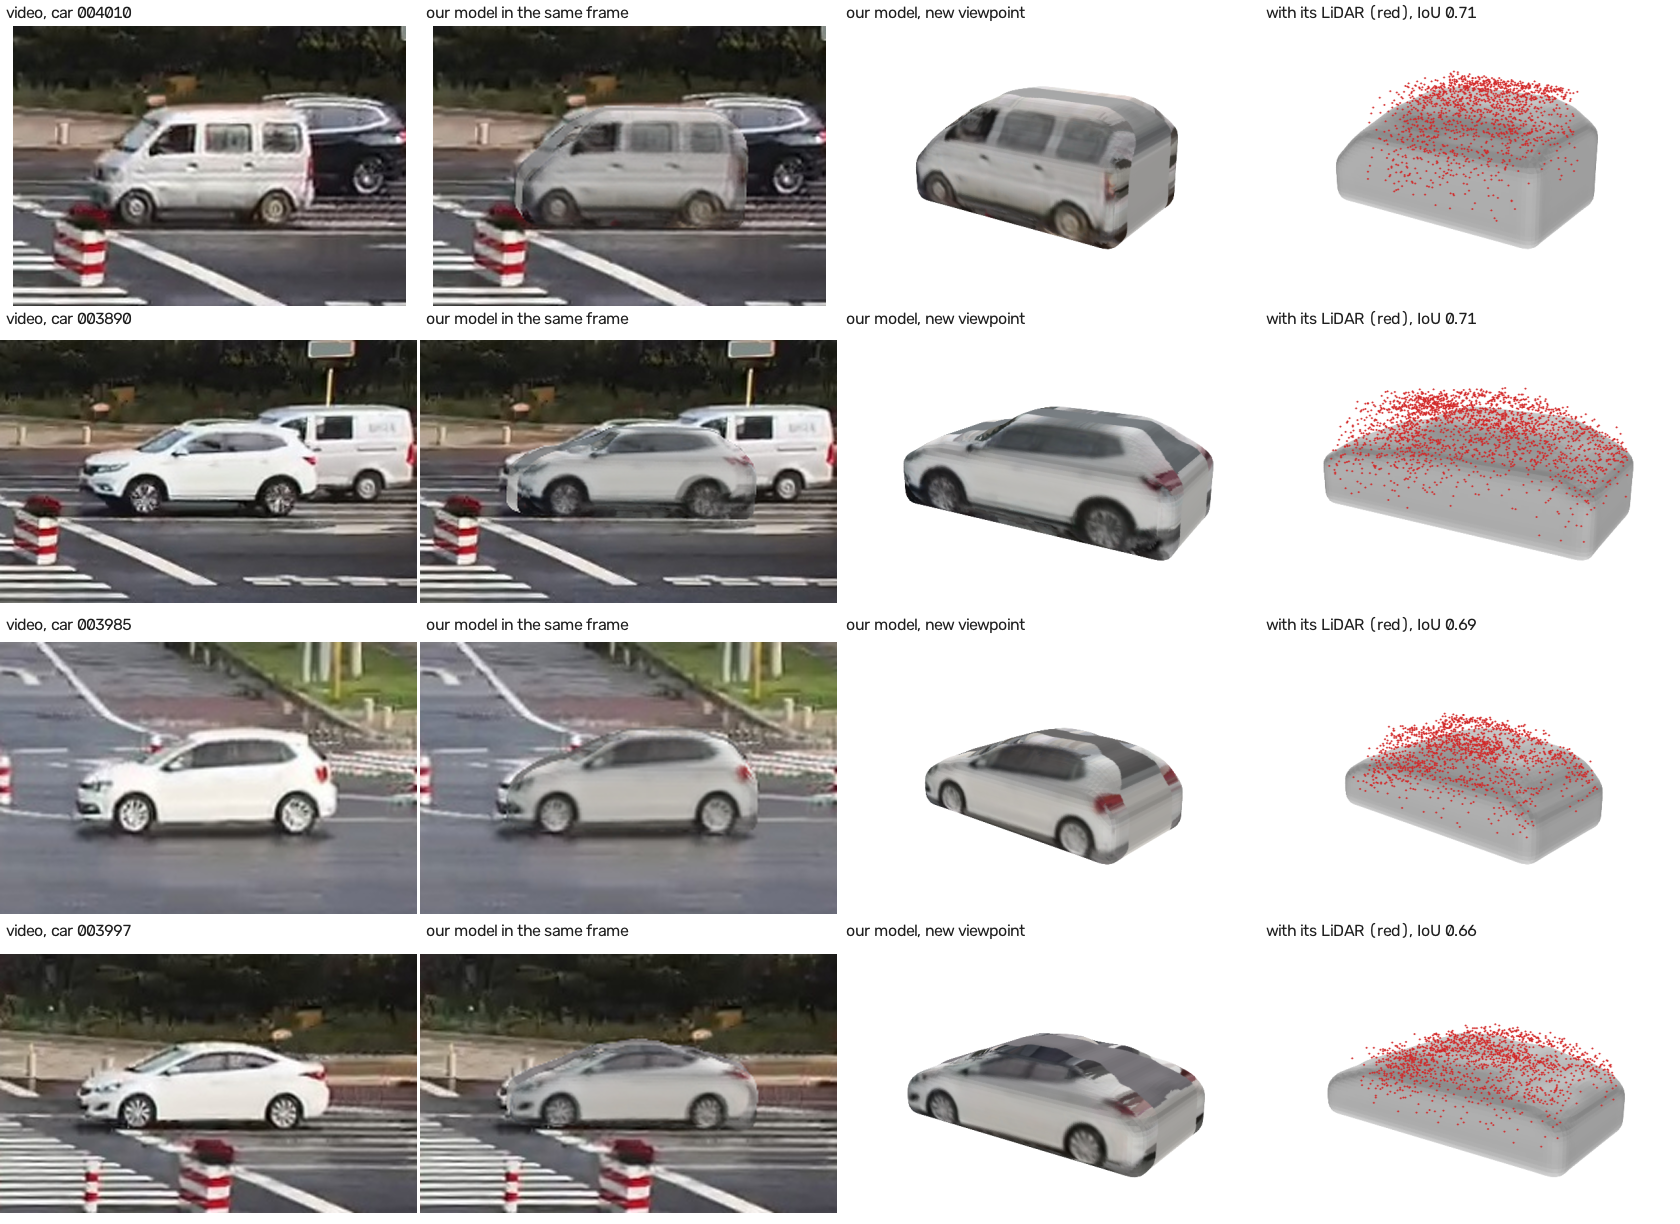
\includegraphics[width=\textwidth]{cars_best.png}
\caption{Four cars of intersection A: a van, a hatchback and two sedans, each shown in a frame where it is
unoccluded. Left to right: the video; our model drawn into the same frame; the model from a
new viewpoint, with the colours of the video pixels; the model with the car's accumulated LiDAR (red, evaluation
only) and the solid IoU against it.}
\label{fig:cars}
\end{figure}

\begin{figure}[!htb]
\centering
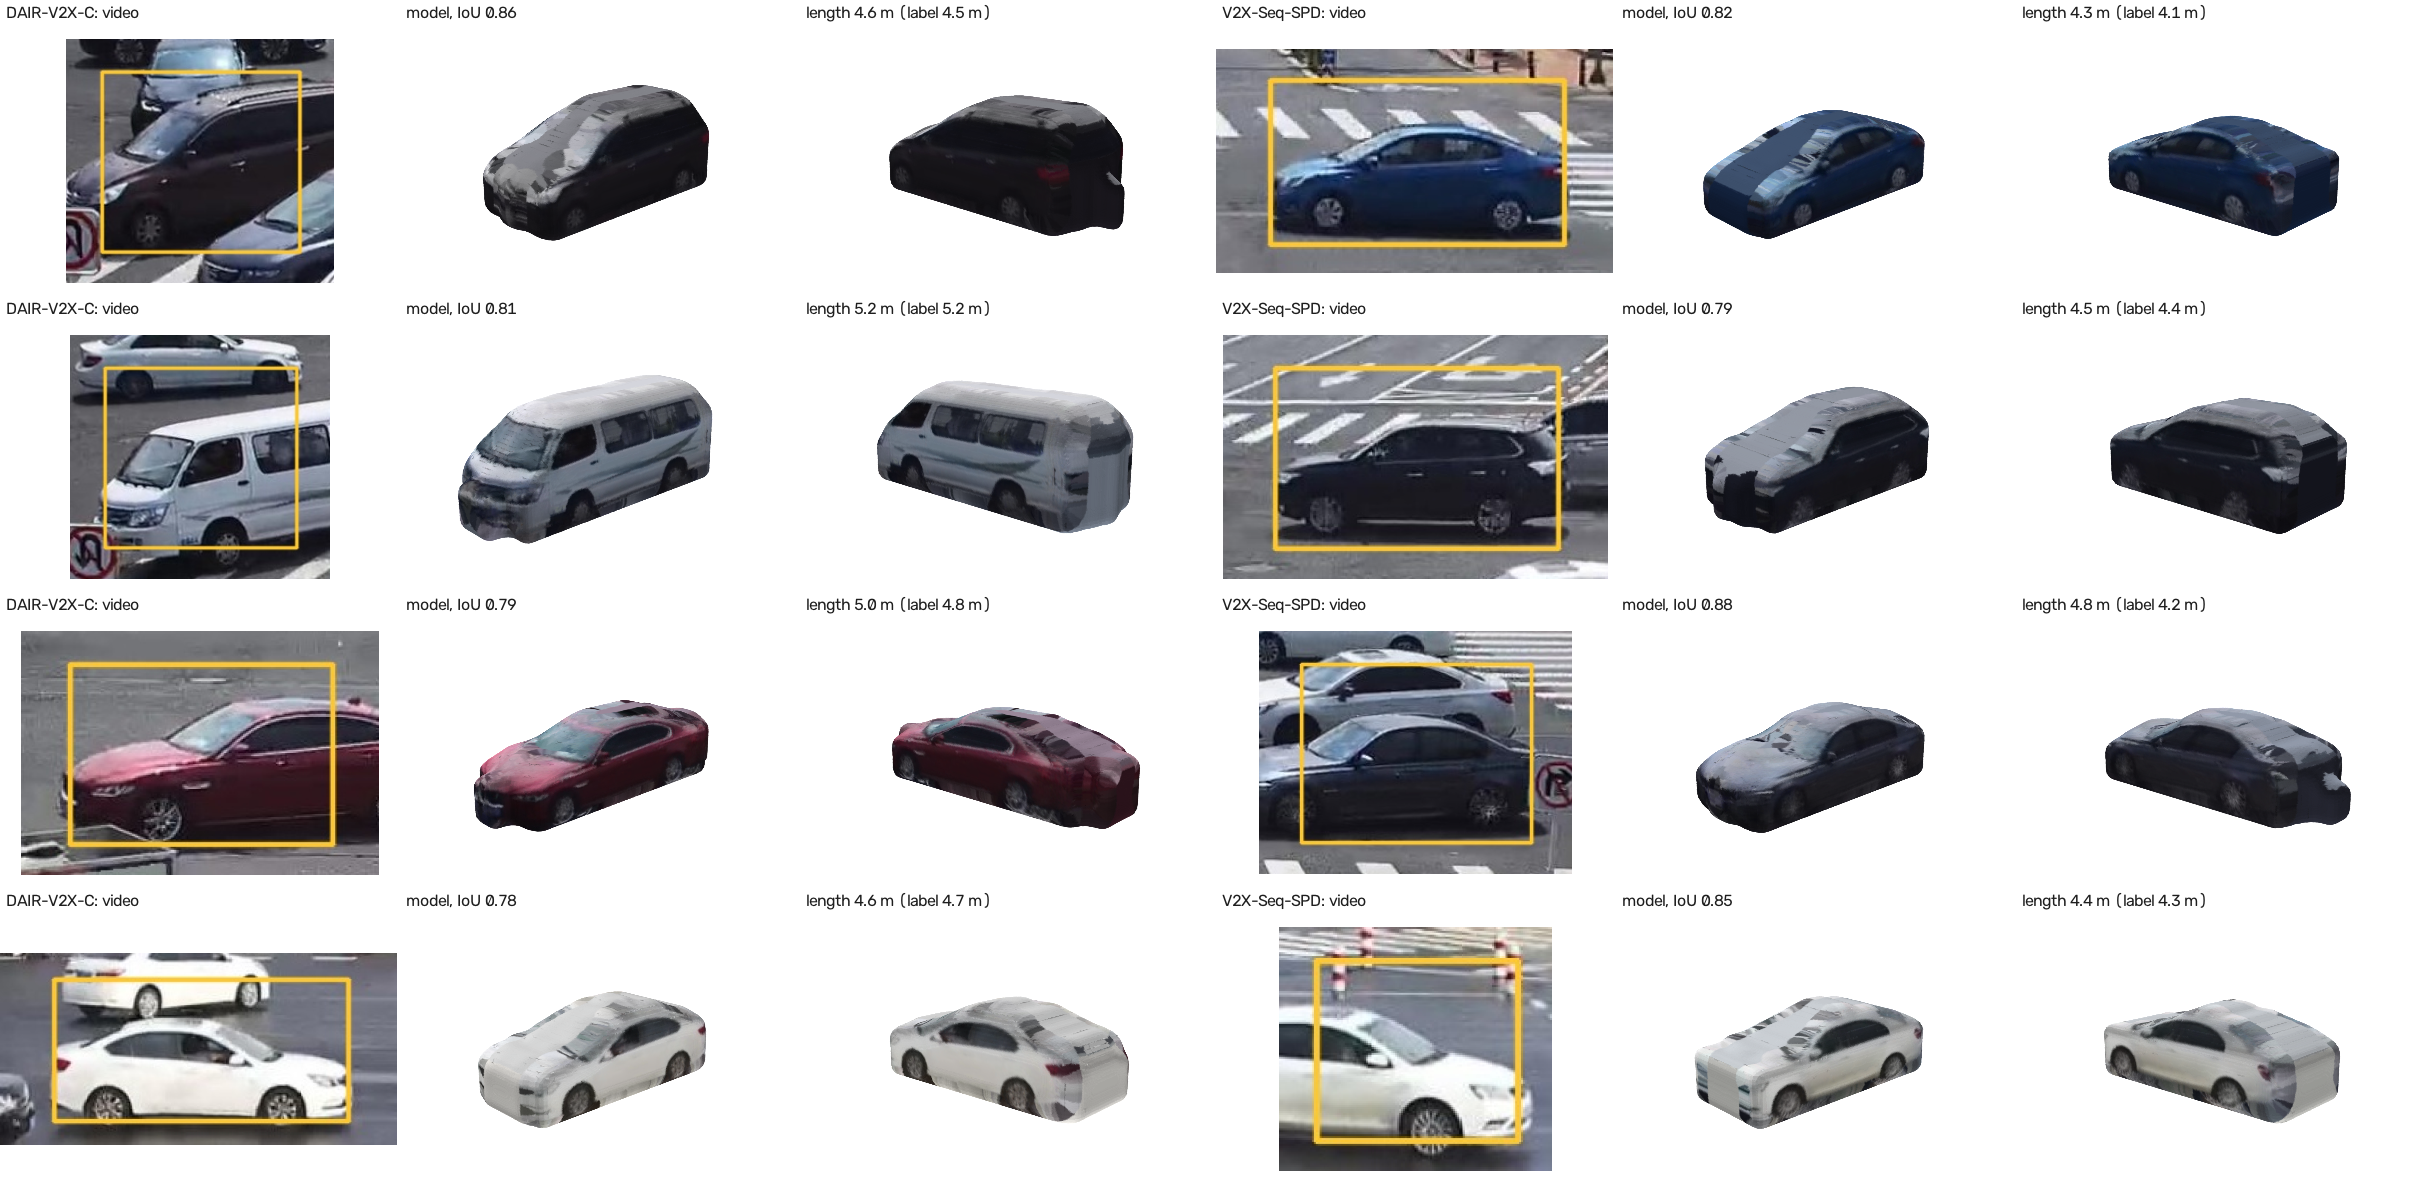
\includegraphics[width=\textwidth]{best_models.png}
\caption{Eight car models of both datasets. Per car: a video frame of the car; the model with the original pixels
of its best views from the front left and from the rear left; its
solid IoU against the gap-closed LiDAR and its length against the labelled length.}
\label{fig:large}
\end{figure}

\paragraph{What limits the result.} Every window is scaled by its cuboid and the cabin is carved from the masks
(Sects.~\ref{sec:window} and~\ref{sec:completion}), so the errors of either go directly into the model. The input cuboids themselves score below the labelled boxes in eight of the nine clips (Table~\ref{tab:clips}), and the models are below their input cuboids in clip 52 and in sequences 0054 and 0002: there the fusion loses against its own input.

\paragraph{The classical input.} Table~\ref{tab:classical} evaluates the classical input of
Sect.~\ref{sec:classical} on all frames of intersections A and B. Of the moving road users within 80~m it finds
39\,\% on A at a precision of 0.67, and 81\,\% at 0.63 on B, where the labels lag the image; in the median the heading
is within $3.5^\circ$ and $1.5^\circ$ and the length within 0.4--0.6~m. Against the cars' accumulated LiDAR its
cuboids score 0.489 on A against 0.544 for the labelled boxes, and 0.432 against 0.437 on B. It fails on touching cars
of one colour and motion, which it takes as one object, on cars whose lower part a car in front hides, and on stopped
vehicles.

\begin{table}[t]
\centering
\caption{The classical input (Sect.~\ref{sec:classical}) on all frames of intersections A and B. Top: against the labelled boxes of the moving road users (at least 1~m/s, within 80~m, not truncated), matched per frame within 3~m (on B within 6~m: its labels lag the image by the camera--LiDAR clock offset, Sect.~\ref{sec:limits}); medians. Bottom: the classical cuboid of each matched car (the median over its frames) and its labelled box against the car's LiDAR accumulated over the clip, scored as in Table~\ref{tab:main} by a re-implementation of the protocol; means, and the paired difference (cuboid $-$ labelled box) with a 95\,\% bootstrap interval. These cars are every labelled car matched to a classical object in at least three frames, with at least 100 LiDAR points: a set other than the reconstructed cars of Table~\ref{tab:main}, on which the labelled boxes therefore score differently.}
\label{tab:classical}
\small
\setlength{\tabcolsep}{4pt}
\begin{tabular}{lcc}
\toprule
 & intersection A & intersection B \\
\midrule
frames & 250 & 83 \\
labelled object-frames & 1851 & 529 \\
recall / precision & 0.39 / 0.67 & 0.81 / 0.63 \\
centre error (m) & 1.64 & 2.33 \\
heading error (mod $180^\circ$) & 3.5$^\circ$ & 1.5$^\circ$ \\
2D box IoU & 0.68 & 0.67 \\
size error $L$ / $W$ / $H$ (m) & 0.61 / 0.22 / 0.18 & 0.42 / 0.18 / 0.25 \\
\midrule
cars against the LiDAR & 32 & 27 \\
solid IoU raw, cuboid / box & 0.361 / 0.393 & 0.323 / 0.323 \\
solid IoU closed, cuboid / box & 0.489 / 0.544 & 0.432 / 0.437 \\
footprint IoU, cuboid / box & 0.59 / 0.75 & 0.53 / 0.59 \\
paired $\Delta$ IoU closed & $-0.055$ $[-0.094, -0.023]$ & $-0.005$ $[-0.053, +0.033]$ \\
\bottomrule
\end{tabular}
\end{table}

% ------------------------------------------------------------------------------------------------------------------
\section{Comparison with Other Approaches}\label{sec:comparison}

There is no common benchmark for car \emph{shapes} from roadside video, and published monocular detectors report the
average precision of boxes, not shape IoU against LiDAR; their numbers are not comparable with ours, and we did not
retrain them. Table~\ref{tab:compare} therefore compares what each family of methods needs and produces.
Quantitatively, the labelled box and the box of our own size in Table~\ref{tab:main} stand in for a perfect and for a
size-only box detector: our shapes are level with both on A and B and below the labelled box on the further clips.

\begin{table}[t]
\centering
\caption{What families of methods need and produce. ``3D labels'': labelled 3D boxes or shapes for training.}
\label{tab:compare}
\setlength{\tabcolsep}{3pt}
\footnotesize
\newcolumntype{L}[1]{>{\raggedright\arraybackslash}p{#1}}
\begin{tabular}{L{3.6cm}L{1.5cm}L{1.6cm}L{1.4cm}L{3.0cm}}
\toprule
family & training data & input & output & main limitation here \\
\midrule
learned box detectors \cite{smoke,monodle,monoflex,fcos3d} & 3D labels & one image & 3D box & no shape; trained per camera type \\
learned roadside detectors \cite{bevheight} & 3D labels & one image & 3D box & no shape; needs roadside labels \\
geometric box lifting \cite{deep3dbox,lift,efficient_orig} & 2D labels or none & one image & 3D box & size prior, no shape \\
learned shape models \cite{kar2015,deepmanta,rcnn3d} & CAD / 3D shapes & one image & shape & shape prior; not shown at 60~m \\
visual hull, space carving \cite{laurentini,spacecarving} & none & many cameras & shape & needs widely spread views \\
multibody SfM \cite{ozden2010,kumar2017} & none & video & points / depth & sparse, no closed shape \\
classical moving-object detection \cite{moving_orig,dubska2014} (Sect.~\ref{sec:classical}) & none & video of a fixed camera & masks, 3D box & merges touching cars of one colour and motion; misses stopped ones \\
\textbf{ours} & none & video of a fixed camera & closed shape & needs motion; length of end-on cars from the cuboid \\
\bottomrule
\end{tabular}
\end{table}

Learned box detectors \cite{smoke,monodle,bevheight} are fast and robust at short and medium range but need
thousands of labelled boxes from comparable cameras and output no shape. Learned shape models
\cite{kar2015,deepmanta,rcnn3d} produce shapes from a single image but need a shape prior learned from CAD models or
3D annotations, and they have not been evaluated at 60~m from a roadside camera. Silhouette methods
\cite{laurentini,spacecarving} need many, widely spread viewpoints; a single high camera gives a narrow range of
directions per car, which is why our visual hull alone over-estimates the height and the length of cars seen end-on.
Our method uses the motion of the car itself to obtain the views that a static multi-camera setup would provide, and
uses the textured body for depth where silhouettes are ambiguous; it needs no training data, but it needs a fixed,
calibrated camera and enough motion, and it reconstructs a car only after it has been tracked for about two seconds.

% ------------------------------------------------------------------------------------------------------------------
\section{Limitations}\label{sec:limits}

\begin{itemize}
\item \emph{Input.} The reconstruction is only as good as its masks and cuboids. With the classical input the models
  are level with the labelled boxes on A and B and below them on the further clips, and they do not improve on their
  own input cuboids (Table~\ref{tab:main}). The classical input misses or merges cars in dense traffic
  (Table~\ref{tab:classical}), so that \ClsACars{} of the 24 cars of A get a model; a stronger detector and segmenter
  can replace it, which we did not evaluate. Stopped objects have no parallax and are not reconstructed.
\item \emph{Sample.} \ClsTotalCars{} cars are scored, eight and nine of them on the two intersections; the
  intervals are wide, and there is no ablation of the parts of the method on this input.
\item \emph{Slow cars.} A car that creeps through the intersection for a long time is seen in many windows whose
  small misalignments along its path add up, and it comes out too long.
\item \emph{Completion.} A car never seen side-on, typically one seen only from behind, takes its length from the
  cuboid and its profile from its body type: its length is not measured from the video.
\item \emph{Synchronisation.} Where camera and LiDAR are not synchronised (intersection B), the model, valid at the
  camera's time, is offset along the path from the label, valid at the LiDAR's; the shape, compared in the car's own
  frame, is not affected, the position is.
\item \emph{Tuning.} The parameters were chosen on intersection A with more precise masks and cuboids than the
  classical ones, and B and clips of the two datasets informed three choices (Sect.~\ref{sec:protocol}); no set is a
  clean hold-out. All intersections are in one city, the two datasets share them, and all use the same kind of camera.
\item \emph{Other road users.} Only cars are evaluated. Pedestrians and cyclists are thin and partly non-rigid, and
  the classical input finds them in too few frames; they are left to future work.
\item \emph{Run time.} The reference Python implementation needs one to two minutes per window on a single CPU core and a
  few minutes per car for the track solve; the classical input takes about 6~s per frame (the 250 frames of A in
  about 25 minutes). Neither is optimised.
\end{itemize}

% ------------------------------------------------------------------------------------------------------------------
\section{Conclusion}

From a single fixed, elevated roadside camera, the 3D shapes of the cars that move past it can be triangulated from
the video alone, with no learned step: the masks and cuboids come from a classical method, and the reconstruction
adds the shape inside the cuboid. Measured against the cars' own LiDAR at up to 70~m, the models are level with the
labelled 3D boxes on the two intersections the method was developed on (\ClsAOurs{} against \ClsALab{}, and
\ClsBOurs{} against \ClsBLab{}) and below them on \ClsDCars{} cars of DAIR-V2X-C and \ClsSCars{} cars of
V2X-Seq-SPD; they are far ahead of a single window, and they do not yet improve on their own input cuboids. Three
ingredients carry the reconstruction: the object's own motion, which turns one camera into many views of its
textured surface; all frames that see the object, solved as one rigid body and completed by symmetry and by the
masks' carve; and, only where the video never measured the length, the cuboid. Its result follows the quality of the
masks and cuboids, which is where the chain from the video alone has the most to gain. The evaluation also shows
that the raw accumulated LiDAR is a biased reference at long range and should be closed before it is used to
compare shapes.

\backmatter

\section*{Abbreviations}
CAD: computer-aided design; IoU: intersection over union; IPM: inverse perspective mapping; LiDAR: light detection and ranging; RANSAC:
random sample consensus; SUV: sport utility vehicle; V2X: vehicle-to-everything.

\section*{Declarations}

\bmhead{Availability of data and materials}
The datasets analysed during the current study are available from their providers after registration: V2X-Seq
\cite{v2xseq} and DAIR-V2X \cite{dairv2x}. The code behind the method, the tables and the figures is available in the
GitHub repository RoadsideCarShape \cite{code}.

\bmhead{Competing interests}
The author declares no competing interests.

\bmhead{Funding}
This research received no funding.

\bmhead{Authors' contributions}
DZ conceived and designed the study, implemented the method, performed the experiments and wrote the manuscript. The
author read and approved the final manuscript.

\bmhead{Acknowledgements}
Not applicable.

\bibliography{references}

\end{document}
